\section{Предварительные замечания}

Единственным фактом из теории представлений, который нам потребуется, будет тот, что групповая алгебра $\mathbb{C}[G]$ конечной группы $G$ разлагается в прямое произведение $\mathbb{C}[G] \cong \mathbb{C}^{d_1 \times d_1} \times \dotsm \times \mathbb{C}^{d_k \times d_k}$ матричных алгебр порядков $d_1, \dotsc , d_k$. Эти порядки являются \hyperref[def:characters_degree]{степенями характеров} $G$, то есть размерностями неприводимых представлений. Из подсчёта размерностей справа и слева следует, что $|G| = \sum_id_i^2$. Также легко доказать, что если $G$ имеет абелеву подгруппу $A$, тогда все степени характеров $G$ меньше или равны индексу $|G:A|$ (утверждение 2.6 в \cite{huppert1998}).

Следующая лемма потребуется нам несколько раз.
\begin{lemma}\label{lem:05:1.1}
  Пусть $s_1, s_2, \ldots, s_n$ неотрицательные действительные числа и положим, что для любого вектора $\mu = (\mu_1, \ldots, \mu_n)$ неотрицательных целых чисел, для которых $\sum_{i=1}^n \mu_i = N$ мы имеем
\[
	{{N}\choose{\mu}} \prod\limits_{i=1}^n s_i^{\mu_i} \leq C^N.
\]
Тогда $\sum_{i=1}^{n} s_i \leq C$.
\end{lemma}
\begin{proof}
	Для любого распределения вероятностей $p=(p_1,\ldots,p_n)$ мы можем устремить $N$ в бесконечность и выбрать $\mu$ так, что $\lim_{N \to \infty} \mu/N = p$.

	Из условия леммы 
	\[
		 {N \choose \mu} \prod\limits_i s_i^{\mu_i} \leq C^N.
	\]
	После извлечения $N$-ого корня получим
	\begin{equation}\label{eq:03:1}
		{N \choose \mu}^{1/N} \prod\limits_i s_i^{\mu_i \over N} \leq C.
	\end{equation}
	Так как
	\begin{align*}
	  \ln {N \choose \mu}^{1/N} & =  \frac{1}{N} \ln \frac{N!}{\mu_1! \dotsm \mu_n!}\\
	  & =  \frac{1}{N} \left( \ln N! - \sum_i \ln \mu_i! \right)\\
	  & \geq  \frac{1}{N} \left( N \ln N - \cancel{N} - \sum_i \mu_i \ln \mu_i + \cancel{\sum_i \mu_i} \right) \text{ (по формуле Стирлинга) }\\
	  & =  \frac{1}{N} \ln \frac{N^N}{\prod_i \mu_i^{\mu_i}} = \frac{1}{N} \ln \frac{\prod_i N^{\mu_i}}{\prod_i \mu_i^{\mu_i}} = \frac{1}{N} \ln \prod_i \left( \frac{N}{\mu_i} \right)^{\mu_i} = \frac{1}{N} \sum_i \mu_i \ln \frac{N}{\mu_i}\\
	  & =  -\sum_i \frac{\mu_i}{N} \ln \frac{\mu_i}{N},
	\end{align*}
	то после взятия натурального логарифма из \eqref{eq:03:1} и устремления $N$ в бесконечность получится
	\[
		-\sum\limits_i p_i \ln p_i + \sum\limits_i p_i \ln s_i \leq \ln C.
	\]
	Положив $S = \sum_i s_i$ и $p_i = s_i / S$, получим
	\begin{align*}
	     -\sum\limits_i p_i \ln p_i + \sum\limits_i p_i \ln S p_i & = -\cancel{\sum\limits_i p_i \ln p_i} + \cancel{\sum\limits_i p_i \ln p_i} + \ln S \sum\limits_i p_i\\
	     & =\ln S \leq \ln C.
	\end{align*}
	В итоге получим, что $S \leq C$.
\end{proof}

Иногда будет нужно оценивать степени характеров у \hyperref[def:wreath_product]{сплетений}.

\begin{lemma}\label{lem:05:1.2}
  Пусть $\{ d_k\}$ степени характеров конечной группы $H$ и пусть $\{ c_j\}$ --- степени характеров $S_n \ltimes H^n$ (где $S_n$ действует переставляя координаты). Тогда $\sum_j c_j^\omega \leq (n!)^{\omega-1}\left( \sum_k d_k^\omega \right)^n$.
\end{lemma}
\begin{proof}[Набросок доказательства] 
Когда $H$ --- абелева группа, теорема следует из элементарных фактов, что степени характеров $S_n \ltimes H^n$ не превосходят $n!$ (это индекс $H^n$ в $S_n \ltimes H^n$), и что $\sum_j c_j^2 = |S_n \ltimes H^n|$. Для произвольного $H$, теорема может быть выведена из общеизвестного описания степеней характеров $S_n \ltimes H^n$ (смотри, например, теорему 25.6 в \cite{huppert1998}).
\end{proof}

Одна конструкция будет особенно полезна. Она включает в себя перестановки точек в треугольном массиве. Пусть
\[
	\Delta_n=\{ (a, b, c) \in \mathbb{Z}^3 \mid a+b+c=n-1 \mbox{ и } a,b,c \geq 0 \}.
\]
Геометрически эти тройки являются барицентрическими координатами для треугольного массива точек с $n$ точками вдоль каждой из сторон, например, для $n=5$ массив будет выглядеть следующим образом, сверху над точками указаны соответствующие элементы из $\Delta_n$:
\begin{figure}[H]
	\centering
    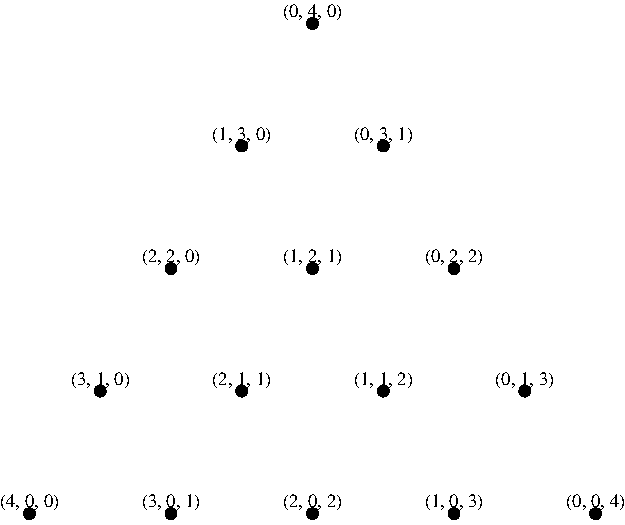
\includegraphics[width=0.45\textwidth]{figures/triangle_array_with_labels}
	\caption{Треугольный массив точек}
	\label{fig:triangle_array_with_labels}
\end{figure}
Взглянув на этот рисунок, можно легко подсчитать количество элементов в $\Delta_n$:
\[
	|\Delta_n| = 1 + 2 + \dotsb + n = \frac{n (n + 1)}{2}.
\]

Для $x \in \Delta_n$ будем писать $x = (x_1,x_2,x_3)$. Пусть $H_1, H_2, H_3$ подгруппы $S_{\Delta_n}$, которые сохраняют первую, вторую и третью координаты соответственно. А именно,
\[
	H_i = \{ \pi \in  S_{\Delta_n} \mid (\pi(x))_i = x_i \mbox{ для всех } x \in \Delta_n\}.
\]

\begin{theorem}\label{th:05:1.7}
  Подгруппы $H_1, H_2, H_3$, определённые выше, удовлетворяют свойству тройного произведения.
\end{theorem}
\begin{proof}
	Пусть $h_1h_2h_3=1$ с $h_i \in H_i$. Упорядочим тройки лексикографически так, что $(0,0,n-1)$ --- наименьшая тройка, а $(n-1,0,0)$ --- наибольшая, и докажем по индукции, что $h_1, h_2$ и $h_3$ фиксируют любую тройку.

	Предположим, что любая из перестановок $h_1, h_2$ и $h_3$ оставляет на месте все тройки меньше $(a,b,c)$ (в базовом случае множество таких троек пустое). Перестановка $h_3$ не может перевести  $(a,b,c)$  в меньшую тройку, так как все меньшие тройки зафиксированы, поэтому $h_3$ должна перевести её в $(a+i, b-i, c)$, где $i \geq 0$. Затем $h_2$ переводит её в $(a+i+j, b-i, c-j)$ для какого-то $j$.

	$h_1$ сможет вернуться к $(a,b,c)$ только если $i+j=0$, значит так оно и есть. Однако $h_1$ оставляет на месте $(a,b-i,c+i)$ для $i \geq 0$ (потому как такая тройка меньше чем $(a,b,c)$) поэтому $i=0$. Отсюда следует, что $(a,b,c)$ фиксируется каждым из $h_1, h_2, h_3$, поэтому по индукции все тройки зафиксированы, то есть $h_1=h_2=h_3=1$. 
\end{proof}
